%!TEX root = ../report.tex
\chapter{ROS Nodes Structure} % (fold)
\label{chap:ros_nodes_structure}
The ROS nodes structure implemented and its topics is shown in the figure \ref{fig:ros_nodes}. The nodes and their explanation are:
\begin{enumerate}
	\item \textbf{Ball tracker}. This node receive image from the camera in its compressed format, extract the same feature in both images and calculate its position in the 3D space. This point is then published. This node is explained in the chapters of $Feature\ extraction$ [\ref{chap:feature_extraction}] and $Stereopsis$ [\ref{chap:stereopsis}].
	\item \textbf{Kalman filter}. The new point is used to predict its future state based on its position and velocity. This nodes lets the robot keep moving even when the cameras have lost the object. The node is defined in the $Prediction$ chapter [\ref{chap:prediction}].
	\item \textbf{Path planning}. Once we have the point located in the space, a new robot's configuration is calculated so the robot can keep the object in sight. The node is explained in the chapter $Path\ planning$ [\ref{chap:path_planning}].
	\item \textbf{Points server}. An auxiliary node has been developed for introduce virtual points in the system so it can be tested in a more modular way.
	\item \textbf{RobWork Studio plugin}. To improve the visioning of the robot and its movements, a real-time viewer plugin has been developed. This plugin allows the user, not only see the robot in its real configuration, but also the tracked object and other geometries.
	\item \textbf{Log}. A new log node has been implemented for our task. This nodes get subscribed to the topics to be logged and plots in real time along as generate graphics for future analysis.
\end{enumerate}

\begin{figure}[!ht]
	\centering
	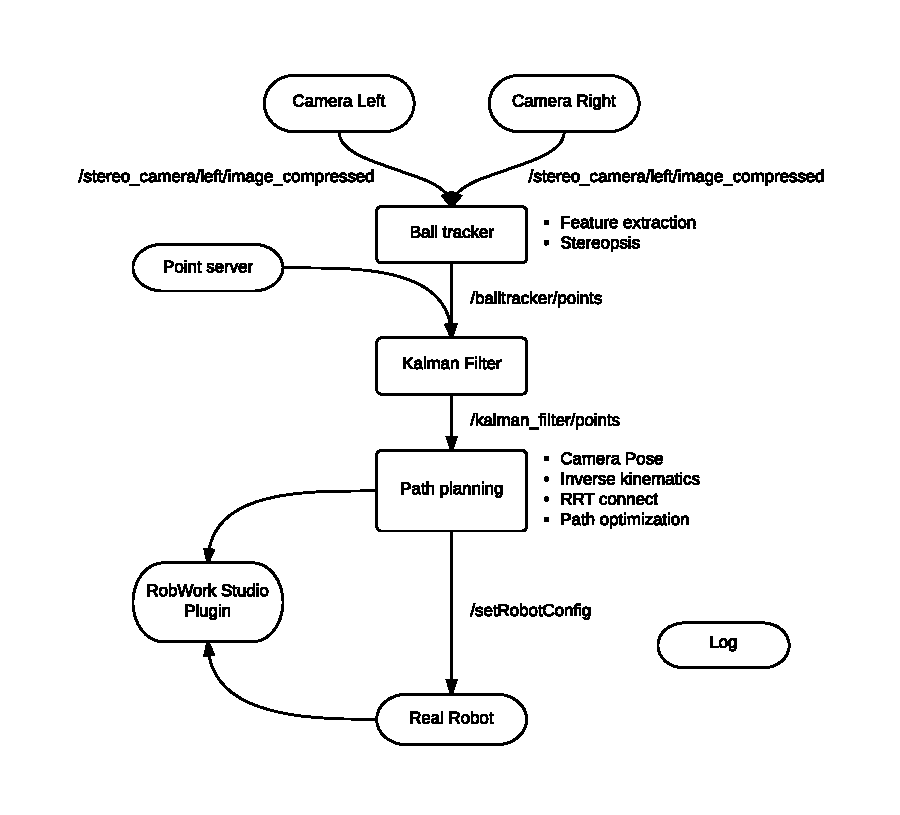
\includegraphics[width=\textwidth]{figures/ros_nodes}
	\caption{ROS Nodes implemented}
	\label{fig:ros_nodes}
\end{figure}
% chapter ros_nodes_structure (end)